%%%%%%%%%%%%%%
%					%
%	INTRODUCCIÓN	%
%					%
%%%%%%%%%%%%%%
\chapter{Introducción}\label{cap:intro}

%Historia de \ecommerce

Una de las actividad mas populares en la \web es comprar. La razón es por que tiene un encanto especial - puedes comprar en tiempo libre, cualquier momento, incluso usando pijamas. Literalmente cualquiera puede tener páginas para mostrar sus productos y servicios.

La historia de \ecommerce se remonta a la invención de la básica noción de “ vender y comprar ”, electricidad, cables, computadores, \textit{modems}, y la \internet. \ecommerce se hace posible en 1991 cuando la \internet estuvo disponible para uso comercial. Desde entonces miles de negocios se han establecido en sitios \web.

En un inicio, el termino \ecommerce se refería al proceso de ejecución  de transacciones electrónicas comerciales con la ayuda de tecnologías lideres tales como \edimeaning y \eftmeaning las cuales dieron la oportunidad a los usuarios para intercambiar información de negocios y realizar transacciones electrónicas. La oportunidad para utilizar estas tecnologías surgió a finales de 1970s y permitió a los negocios de las compañías y organizaciones enviar documentación electrónica comercial.

Aunque la \internet comenzó a ganar popularidad  entre el publico general en 1994, tomó aproximadamente cuatro años desarrollar protocolos de seguridad ( por ejemplo \http) y DSL los cuales permitieron un acceso rápido y conexiones persistentes a la \internet. En 2000 un gran número de empresas comerciales en los Estados Unidos y Europa Occidental presentaron sus servicios en la \www. En ese entonces el significado de la palabra \ecommerce fue cambiado. Las personas comenzaron a utilizar el termino \ecommerce como el proceso de compra de productos y servicios disponibles en \internet utilizando conexiones seguras y servicios de pago electrónico. Aunque el colapso de \dotcom en 2000 dirigió a desafortunados resultados y muchas compañías \ecommerce desaparecieron, los \retailers \brickandmortar reconocieron las ventajas del comercio electrónico y comenzaron a la integración de tales características a sus sitios \web. Para finales de 2001, el modelo de negocio mas grande de \ecommerce, \btob, había ganado al rededor de \$700 billones en transacciones.

\begin{figure}[h!]
	\centering
	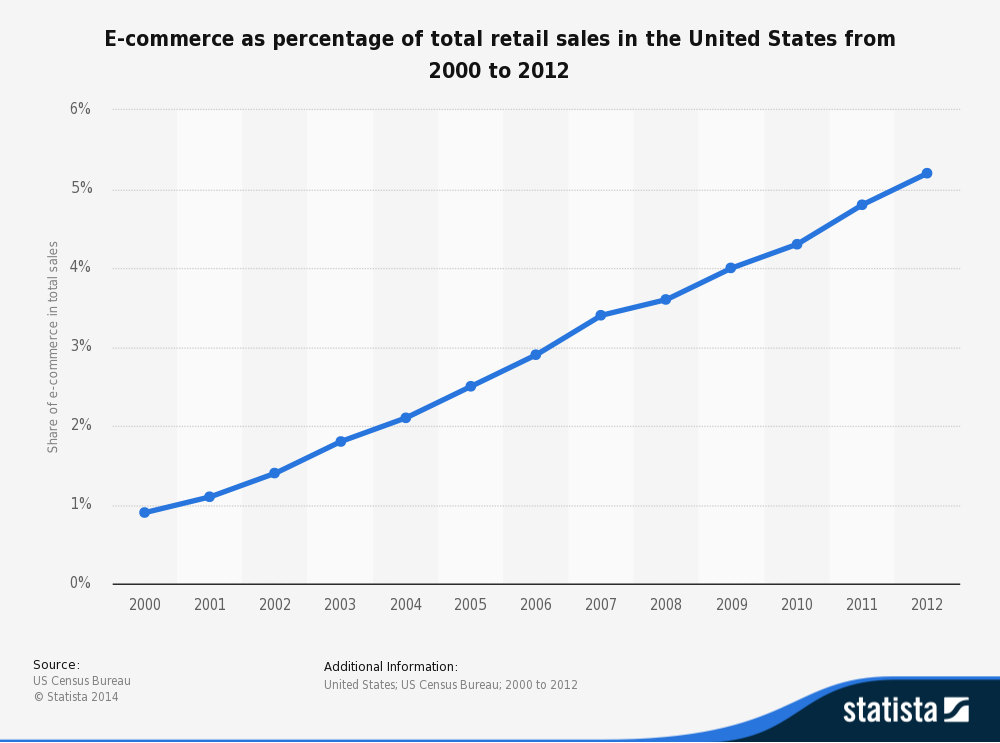
\includegraphics[width=0.7\textwidth]{figuras/ecommerce_percent.jpg}
	\caption{\ecommerce como porcentaje de las ventas totales en Estados Unidos}
	\label{figure:ecommerce_percent_sales}
\end{figure}

Acorde a toda información disponible, las ventas \ecommerce continuaron creciendo en los siguientes años y, en 2012 las ventas \ecommerce representaron el 5.2\% de las ventas totales en el mundo. Como se puede observar en \refFigura{figure:ecommerce_percent_sales}.

\ecommerce tiene muchas ventajas sobre tiendas \brickandmortar y catálogos de venta por correo. Los consumidores pueden fácilmente buscar a través de una base de datos muy extensa de productos y servicios. Pueden ver los precios reales, definir una orden de compra en varios días y enviar un correo como un \wishlist esperando que alguien pague por sus productos seleccionados. Los clientes pueden comparar precios con un simple \click del \mouse y comprar los productos seleccionados al mejor precio.

Proveedores \online, en sus turnos, también tienen claras ventajas. La \web y sus motores de búsqueda proveen una manera para encontrar clientes sin campañas de publicidad costosas. Incluso tiendas \online pequeñas pueden alcanzar mercados globales. 

La tecnología \web también permite realizar un seguimiento sobre las preferencias de los clientes para ofrecer una comercialización personalizada.

%La historia de \ecommerce is impensable sin Amazon e Ebay los cuales estuvieron entre las primeras compañías que permitían transacciones electrónicas. Gracias a sus fundadores ahora tenemos un sector considerable de \ecommerce y disfrutar de comprar y vender gracias a la Internet. Actualmente hay 5 de los mas grandes y mas famosos \textit{worldwide internet retailers}: Amazon, Dell, Staples, Office Depot y Hewlett Packard. De acuerdo a las estadísticas, las categorías de productos mas vendidos en \textit{Worl Wide Web} son música, libros, computadores, artículos de oficina y otros dispositivos electrónicos.
%
%Amazon.com, Inc. es uno de las mas famosas compañías \ecommerce  para vender productos sobre la Internet. Después del colapso \textit{dot-com} Amazon perdió su posición de modelo de negocio exitoso, sin embargo, en 2003 la compañía hizo su primer año con utilidades el cual fue el primer paso para el desarrollo futuro.
%
%Al principio Amazon.com fue considerado como una tienda \textit{online} de libros, pero con el tiempo una variedad de productos electrónicos fueron agregados, software, DVDs, juego de video, CDs de música, MP3s, prendas de vestir, calzado, productos de salud, etc. El nombre original de la compañía fue Cadabra.com, pero rápidamente después que se volviera popular Internet Bezos decidió cambiar el nombre de su negocio a “Amazon” después del río voluminoso mas grande del mundo. En 1999 Jeff Bezos fue nombrado como la persona del año por Time Magazine en reconocimiento al éxito de la compañía. Aunque la sede principal de la empresa se encuentra en USA, WA, Amazon ha establecido sitios \textit{web} separados en otros países tales como United Kingdom, Canada, France, Germany, Japan, y China. La compañía apoya y opera \textit{retail web sites} para muchos negocios famosos, incluyendo Marks \& Spencer, Lacoste, la NBA, Bebe Stores, Target, etc.
%
%Amazon es uno de los primeros negocios \ecommerce en establecer un programa de marketing para los afiliados, y actualmente la compañía obtiene cerca del 40\% de sus ventas desde afiliados y vendedores de terceras partes que lista y vende productos en el sitio \textit{web}. En 2008 Amazon penetro en el cine y actualmente esta patrocinando la película \textit{“The Stolen Child”} con \textit{20th Century Fox}.
%
%Acorde a las investigaciones en 2008, el dominio Amazon.com a traído cerca de 615 millones de clientes cada año. La característica mas popular del sitio \textit{web} es el \textit{review sistem}, i.e., la habilidad de los visitantes de presentar sus \textit{reviews} y \textit{rate} cualquier producto en un \textit{raiting scale} de uno a 5 estrellas. Amazon.com es también \textit{well-know} por su \textit{clear and user-friendly} avanzado sistema de búsqueda que permite a los visitantes buscar por \textit{keywords} en el texto completo de muchos libros en la base de datos.
%
%Otra compañía ha contribuido mucho en el proceso de desarrollo de \ecommerce es Dell Inc., una compañía americana posicionada en Texas, que se sitúa en el tercer lugar de ventas de computadoras después de Hewllett-Packard y Acer.
%
%Lanzado en 1994 como una pagina estática, Dell.com ha realizado rápidos pasos, y para finales de 1997 fue la primera compañía en lograr el \textit{record} de un millón de ventas \textit{online}. Su única estrategia de ventas sobre la \textit{World Wide Web} sin \textit{retail outlets} y sin intermediarios ha sido admirado por un sin fin de clientes e imitado por un gran numero de \ecommerce \textit{businesses}. El factor de éxito de Dell es que Dell.com permite a los clientes elegir y controlar, i.e., visitantes pueden explorar el sitio y ensamblar PC pieza por pieza eligiendo el mas mínimo componente basado en sus presupuestos y requerimientos. De acuerdo a las estadísticas, aproximadamente la mitad de las ganancias de las compañías proviene desde su sitio \textit{web}.
%
%En 2007, Fortune magazine \textit{ranked} Dell como la \textit{34th-largest} compañía en \textit{Fortune 500 list}, y \textit{8th} en su \textit{Top 20 list} anual de las mas exitosas y admiradas compañías en USA en reconocimiento al \textit{bussiness model} de la compañía.

La historia de \ecommerce es nueva, un mundo virtual que esta evolucionando de acuerdo a las ventajas del cliente. Es un mundo que todos construyen en conjunto ladrillo por ladrillo, estableciendo una base segura para las nuevas generaciones.

\subsection{\ecommerce en la actualidad}

En la actualidad, \ecommerce es una experiencia destacable. Transformo las compras tradicionales mas allá de lo reconocible. La experiencia es mucho mejor que cualquier otra manera de comprar, seduciendo a una gran cantidad de \ecommerce \lovers.

Si hace algunos años atrás \ecommerce fue una palabra de moda, ahora se ha convertido en la orden del día. Al parecer las personas compran literalmente en cualquier parte - en sus lugares de trabajo, durante el almuerzo, en las horas punta cuando no hay nada mas por hacer salvo encender el computador y comenzar a navegar.

En el presente, \ecommerce ha ganado tanta popularidad debido a que su tecnología subyacente esta evolucionando a pasos agigantados. Incluso se esta ofreciendo \textit{"sentir"} el producto con un \mouse \textit{3D} para comprender mejor su forma, tamaño y textura. ¿Para que salir cuando todo lo que se debe hacer es realizar un pedido, elegir la forma de envío, pararse y esperar hasta que la orden sea entregada hasta la puerta?

\ecommerce hoy ofrece tanto lujo que incluso las tiendas convencionales han encendido las alarmas. Aunque, cada uno esta de acuerdo que hay un gran camino para que \ecommerce reemplace las tiendas, la posibilidad existe que ocurra en el futuro. \ecommerce del cual somos actualmente testigos trae tanta aventura a nuestras vidas que es disfrutado por toda la comunidad \online.

En la actualidad \ecommerce tiene algunos inconvenientes; pero quien no se arriesga, no cruza el río. Muchos consumidores están dispuestos a aguantar estas desventajas, ya que confían en el mundo \online y desean que sea un mejor lugar.

\ecommerce en la actualidad refleja lo que hemos creado desde un inicio para el comercio electrónico \online. Fue creado por nosotros y pensado para nosotros.

\subsection{\ecommerce en el futuro}

Expertos predicen un futuro prometedor y glorioso para \ecommerce. En un presumible futuro \ecommerce se confirmara por si misma como una herramienta importante para las ventas. El éxito de \ecommerce se convertirá en una noción inseparable de la \web ya que \eshopping se esta volviendo cada vez mas y mas popular y natural. Al mismo tiempo la competitividad en el mundo de los servicios \ecommerce intensificará su crecimiento. Así la tendencia que  prevalecerá \ecommerce será el crecimiento de las ventas por \internet y la evolución.

Cada año el numero de ofertas de \ecommerce crece enormemente. El volumen de ventas de las tiendas \online  son mas que comparables con esos \brickandmortar. Y la tendencia va a continuar, porque hay mucha gente \textit{encarcelada} por las obligaciones laborales y de los hogares, mientras que \internet permite ahorrar mucho tiempo y dinero al permitir  elegir los productos a los mejores precios. Hoy en día el auge de las ventas por \internet es la base del magnífico futuro \ecommerce.

La tendencia \textit{cantidad a calidad} del \ecommerce se está convirtiendo cada vez más evidente, ya que \internet ha incluido el factor geográfico de la venta. Así que no importa más si su tienda se encuentra en New York, Londres o en una pequeña ciudad. Para sobrevivir, los comerciantes tendrán que adaptarse rápidamente a las nuevas condiciones. Para atraer a más clientes, los propietarios de las tiendas \online tendrán no solo que incrementar el número de servicios disponibles, ademas deberán poner más atención a elementos como \design atractivo, \userfriendliness, presentación atractiva; tendrán que oportunamente emplear tecnología moderna para que sus negocios sean parte del futuro del \ecommerce.

Claramente, aquellos que adquieren \estores antes, tienen mejores oportunidades  para el éxito y prosperidad, aunque un sitio \ecommerce por si mismo no garantiza nada. Solo una apropiada solución \ecommerce en combinación con \emarketing y \advertising pueden asegurar éxito.

%TODO INICIO [TEXTO INTRO]: texto inicialmente agregado solo por mi. Mejoras continuas son necesarias

En el mundo de empresarial, el tamaño importa, pero ni siquiera eso garantiza un futuro en un mercado de constante cambio y con una competencia feroz. Innumerables son las empresas que murieron en el intento, entre las cuales podemos destacar : \sega, \kodak, \daewoo, \nokia, \blockbuster, entre otros.

En otras palabras se demanda tener un \ecommerce con la flexibilidad necesaria para posibles cambios en el futuro, así como para soportar una serie de cualidades actualmente disponibles para diferentes tipos de sitios \ecommerce. Se desea entonces un \software con un abstracción tal que provea funcionalidad genéricas que puedan ser cambiadas selectivamente agregando código escrito por un desarrollador, con el fin de obtener un \software \ecommerce con características específicas. En conclusión, lo que se necesita es desarrollar un \ecommerce \framework.

Una aplicación \web es aquella que corre sobre un \web \browser, el cual obtiene los datos que procesa a través de un protocolo estándar de comunicación llamado \http que opera en la \applayer, la cual es parte de \osimodel.

\osimodel es un modelo estándar de arquitectura que constituye el \framework para el desarrollo de protocolos estándar para la interconexión de sistemas. Dicho \framework esta compuesto por 7 \layers que separan las diferentes funcionalidades necesarias(\refFigura{figure:framework_layers_definition})\cite{inbook_osi_reference_model}, de esta forma se divide el problema en partes mas pequeñas.

\begin{figure}[h!]
	\begin{tikzpicture}[node distance=3pt,
		blueb/.style={
	  		draw=white,
	  		fill=mybluei,
	  		rounded corners,
	  		text width=2.5cm,
	  		font={\sffamily\bfseries\color{white}},
	  		align=center,
	  		text height=12pt,
	  		text depth=9pt},
		greenb/.style={blueb,fill=mygreen},
	]

	\node[blueb,text width=13cm+26pt] (APP) {\applayer};
	\node[blueb,below=of APP,text width=13cm+26pt] (PRES) {\preslayer};
	\node[blueb,below=of PRES,text width=13cm+26pt] (SESSION) {\sessionlayer};
	\node[blueb,below=of SESSION,text width=13cm+26pt] (TRANS) {\translayer};
	\node[blueb,below=of TRANS,text width=13cm+26pt] (NETWORK) {\networklayer};
	\node[blueb,below=of NETWORK,text width=13cm+26pt] (LINK) {\datalinklayer};
	\node[blueb,below=of LINK,,text width=13cm+26pt] (PHYSI) {\physilayer};
	
	\begin{pgfonlayer}{background}
	\draw[blueb,draw=black,fill=mybluei!30] 
	  ([xshift=-8pt,yshift=8pt]current bounding box.north west) rectangle 
	  ([xshift=8pt,yshift=-8pt]current bounding box.south east);
	\end{pgfonlayer}
\end{tikzpicture}

\caption{Arquitectura \osimodel }
	\label{figure:framework_layers_definition}
\end{figure}

La idea básica de separar en \layers, es que cada una de estas agrega valor a los servicios provistos por el conjunto inferior de \layers de tal manera que las \layer que esta en la cúspide del \stack ofrece el conjunto de servicios necesarios para ejecutar aplicaciones distribuidas. Cada una de estas 7 \layers representa a su vez un \framework que define sus funcionalidades propias.

\begin{figure}[h!]
	\begin{tikzpicture}[node distance=10pt,
		blueb/.style={
	  		draw=white,
	  		fill=mybluei,
	  		rounded corners,
	  		text width=2.5cm,
	  		font={\sffamily\bfseries\color{white}},
	  		align=center,
	  		text height=8pt,
	  		text depth=5pt},
		greenb/.style={blueb,fill=mygreen},
	]

	\node[blueb,text width=5cm+10pt] (APP) {\applayer};
	\node[below=of APP] (dummy1) {};
	\node[right=of dummy1] (dummy2) {};
	
	\node[above=of PRES] (dummy3) {};
	\node[right=of dummy3] (dummy4) {};
	\node[blueb,below=of APP,text width=5cm+10pt] (PRES) {\preslayer};
	\path[->] (dummy1) edge node {} (dummy3);
	\path[->] (dummy2) edge node {} (dummy4);
	
	\node[blueb,below=of PRES,text width=5cm+10pt] (SESSION) {\sessionlayer};
	\path[->] (PRES.20) edge node {} (SESSION);
	\path[->] (SESSION.-20) edge node {} (PRES);
	
	\node[blueb,below=of SESSION,text width=5cm+10pt] (TRANS) {\translayer};
	\path[->] (SESSION.20) edge node {} (TRANS);
	\path[->] (TRANS.-20) edge node {} (SESSION);
	
	\node[blueb,below=of TRANS,text width=5cm+10pt] (NETWORK) {\networklayer};
	\path[->] (NETWORK.20) edge node {} (TRANS);
	\path[->] (TRANS.-20) edge node {} (NETWORK);
	
	\node[blueb,below=of NETWORK,text width=5cm+10pt] (LINK) {\datalinklayer};
	\path[->] (LINK.20) edge node {} (NETWORK);
	\path[->] (NETWORK.-20) edge node {} (LINK);
	
	\node[blueb,below=of LINK,,text width=5cm+10pt] (PHYSI) {\physilayer};
	\path[->] (PHYSI.20) edge node {} (LINK);
	\path[->] (LINK.-20) edge node {} (PHYSI);
	
%	\begin{pgfonlayer}{background}
%	\draw[blueb,draw=black,fill=mybluei!30] 
%	  ([xshift=-8pt,yshift=8pt]current bounding box.north west) rectangle 
%	  ([xshift=8pt,yshift=-8pt]current bounding box.south east);
%	\end{pgfonlayer}
\end{tikzpicture}

\caption{Arquitectura \osimodel }
	\label{figure:framework_layers_interaction}
\end{figure}

Lo que se plantea es desarrollar un \framework que se encontrará inmediatamente por sobre el \osimodel (\refFigura{figure:framework_above_osimodel}) para facilitar el desarrollo de aplicaciones, productos y soluciones específicas \ecommerce utilizando un ambiente de \software reusable y universal a través de funcionalidades particulares que son parte de una gran plataforma.

\begin{figure}[h!]
	\begin{tikzpicture}[node distance=3pt,
		blueb/.style={
	  		draw=white,
	  		fill=mybluei,
	  		rounded corners,
	  		text width=2.5cm,
	  		font={\sffamily\bfseries\color{white}},
	  		align=center,
	  		text height=12pt,
	  		text depth=9pt},
		greenb/.style={blueb,fill=mygreen},
	]

		\node[blueb, draw=black, fill=myblueii] (SLCN1) {Solución 1};
		\node[blueb, draw=black, fill=myblueii,right=of SLCN1] (SLCN2) {Solución 2};
		\node[right=of SLCN2] (dummy) {};
		\node[blueb, draw=black, fill=myblueii,right=of SLCN2] (SLCN3){Solución 3};
		\node[blueb, draw=black, fill=myblueii,right=of SLCN3] (SLCN4) {Solución 4};
		\begin{pgfonlayer}{background}
			\draw[blueb,draw=black,fill=mybluei!30] 
  				([xshift=-8pt,yshift=8pt]current bounding box.north west) rectangle 
  				([xshift=8pt,yshift=-8pt]current bounding box.south east);
		\end{pgfonlayer}
\node[blueb, draw=black, fill=myblueii, below=22pt of dummy,text width=13cm+26pt] (ECOMM) {\frameworkname};

		\node[blueb, draw=black, fill=myblueii, below=of ECOMM, text width=13cm+26pt] (OSI) {\osimodel};

\end{tikzpicture}

\caption{Arquitectura general de la plataforma \ecommerce }
	\label{figure:framework_above_osimodel}
\end{figure}

%that actual software is an application running on your PC. It doesn't really “reside” at the application layer. Rather, it makes use of the services offered by a protocol that operates at the application layer, which is called the Hypertext Transfer Protocol (HTTP). The distinction between the browser and HTTP is subtle, but important.

%In computer programming, a software framework is an abstraction in which software providing generic functionality can be selectively changed by additional user-written code, thus providing application-specific software. A software framework is a universal, reusable software environment that provides particular functionality as part of a larger software platform to facilitate development of software applications, products and solutions. Software frameworks may include support programs, compilers, code libraries, tool sets, and application programming interfaces (APIs) that bring together all the different components to enable development of a project or solution.



%TODO END [TEXTO INTRO]

\section{Motivación}\label{cap:intro:motivacion}

\online \retailers están en la cúspide de una forma totalmente nueva de hacer negocios. Ellos tienen una oportunidad única para obtener ventajas significativas en sus respectivos mercados, siempre que entreguen consistentemente una experiencia grata para el consumidor y permita un comportamiento de comercio multicanal único antes que sus competidores. El éxito dependerá en perfeccionar los esfuerzos para abordar las experiencias de clientes centrados en el usuario, reducir el enfoque de los programas más valiosos, y eligiendo estrategias de tecnología adecuada que permitan a los equipos internos ofrecer experiencias escalables optimizadas. Las áreas emergentes a observar son \realtime \retail \analytics, incorporar \socialnetwork en \ecommerce, el continuo éxito de aplicaciones móviles, y herramientas que permitan a \retailers \scale experiencias que dirijan de manera mas efectiva el \merchandising.

%Online retailers are on the cusp of a totally new way of doing business. They have a unique opportunity to gain a significant competitive advantage in their respective markets, provided they consistently deliver a consumer-friendly experience and enable unique multichannel commerce behaviors before their competitors. Success will depend on honing efforts to address user-centric customer experiences, narrowing the focus to the most-valuable programs, and electing the right technology strategy that will enable internal teams to deliver optimized scalable experiences. Areas to watch are the emergence of real-time retail analytics, social-network enabled commerce, the continued success of mobile applications, and tools that will enable retailers to scale “always-targeted” experiences that target merchandising more effectively.

Existen una amplia variedad de escenarios en donde existen soluciones \ecommerce o similares con la potencialidad de ser mejorados permitiendo entrar al mercado con ventajas competitivas. A continuación se describen variados situaciones que tienen gran potencial latente.

\begin{itemize}
	\item \textbf{\shoppingCart}:
	
	\item \textbf{Reclamos ciudadanos}: Un sistema para realizar y gestionar reclamos que estén relacionado principalmente temas sociales con el fin de alertar a la brevedad a los organismos públicos responsables. Ejemplos de uso serian: Calles en mal estado, semáforos en mal estado, semáforos que no tengan un tiempo suficiente para cruzar, cruces peligrosos para peatones, aceras en mal estado, lugares de ruido excesivo, lugares de robos comunes, plazas en mal estado. La idea básica es crear una queja, y que los ciudadanos que consideren que dicha queja los representa, unirse a ella para lograr un volumen crítico para que las autoridades sean consientes del impacto que genera dicha queja.
	
	\item \textbf{Reservas horas medicas:} Un sistema para gestionar las horas medicas que muestre sugerencias de acuerdo a la distancia que se encuentran los especialistas desde la \textit{geo-posicion} del sistema que realiza la solicitud. 
	
	\item \textbf{Consultas de libros en una biblioteca:} Un sistema para consultar la disponibilidad, la cantidad, la posibilidad de reservarlo, e incluso cuando sera devuelto.
	\item \textbf{Catálogo de Moteles}: Un catálogo de moteles de acuerdo a la \textit{geo-posicion} pueden ser listados para determinar las mejores opciones disponibles. Adicionalmente se podría mostrar los horarios disponibles de las habitaciones, e incluso poder generar reservas y pagar la habitación. De esta manera se optimiza el tiempo de los clientes, y los recursos de los proveedores.
	
	\item \textbf{Catalogo de Medicamentos}: Un catalogo completo de los medicamentos oficialmente aceptados podrían ser listados para entregar información relevante de acuerdo a las dosis así como de efectos adversos, si es necesaria una receta, etc. Otra cosa interesante, es dar la opción de mostrar todos los remedios genéricos que existen en el mercado. El escenario ideal seria ademas mostrar el precio de estos, así como la distancia a las droguerías en donde el producto se encuentra disponible.
	
	\item \textbf{Reserva de horas en Registro Civil}: Al menos en Chile, realizar un tramite en el registro civil es sinónimo de una perdida de tiempo absurda solo para ser atendido. Si la reserva de hora puede ser realizada desde cualquier sitio, el sistema se volvería drásticamente mas eficiente.
	
	\item \textbf{Catalogo de Fiestas}: Un catalogo con las fiestas disponibles tanto a la brevedad posible, como en el futuro. Que muestre información relevante.
	
	\item \textbf{Gestor de detalle de cuenta en restaurante}: 
	
\end{itemize}

Todas estas situaciones tienen algo en común, y es que los usuarios desean consultar información para tomar una decisión. El sistema idealmente permite contrastar datos entre diferentes proveedores de servicios similares, así como de aportar con información clara y relevante, para que futuros usuarios puedan tomar una decisión aun mas informados.

Como se puede concluir, el modelo de negocio de estas situaciones es en su mayoría el mismo, solo cambiado la presentación para hacerlo \adhoc a la situación.

\section{Alcances y Objetivo General}\label{cap:intro:alcances}

Desarrollar un \framework \ecommerce que permita mayor flexibilidad y/o disminución de la complejidad, en comparación a las \frameworks actuales, en el desarrollo de soluciones específicas. Lo que implica mayor diversidad de aplicaciones, menor cantidad de recursos humanos y menor tiempo de desarrollo.

\section{Objetivos Específicos}\label{cap:intro:objetivos}
%Dentro de los objetivos específicos se encuentran:
\begin{itemize}
	\item Determinar viabilidad del proyecto.
	\item Determinar la tecnología mas adecuada para el desarrollo del proyecto.
	\item Determinar la arquitectura adecuada para el desarrollo del \framework.
	\item Desarrollar un \ecommerce \framework que permita mayor flexibilidad en soluciones específicas, y disminuir la complejidad de código a fin de obtener soluciones mas rápidas y con menor cantidad de recursos humanos.
	\item Desarrollar al menos una solución utilizando \frameworkname, que permite contrastar las potencialidades con respecto a \frameworks existentes.
	\item Utilizando \frameworkname, desarrollar 3 soluciones específicas.
	\item Determinar, en base a las 3 soluciones desarrolladas, si es efectivo que \frameworkname disminuye la complejidad de desarrollo. 
\end{itemize}

\section{Caracteristicas deseables}\label{cap:intro:alcance}

\begin{table}[h!]
    \tiny
   
\begin{tabular}{ |L{0.6\paperwidth}|L{0.1\paperwidth}|}
\hline
	\task &
	Tiempo
	
\\ \hline
	\textbf{ Agregar \itemCOM}: Agregar un \itemCOM a la tienda.&
	
\\ \hline
	\textbf{ Remover \itemCOM}: Remover un \itemCOM de la tienda.&
	
\\ \hline
	\textbf{ Agregar \itemCOM}: &
	
\\ \hline
	\textbf{ Agregar \itemCOM}: &
	
\\ \hline
	\textbf{ Agregar \itemCOM}: &
	
\\ \hline
	\textbf{ Agregar \itemCOM}: &
	
\\ \hline
	\textbf{ \textit{\dragdrop} manejo de variedad}: Organizar el orden de la variedad de \itemCOM en la tienda con \textit{\dragdrop}.&
	%\textbf{ Drag \& Drop Variant Management:} Arrange order of product's variants in your shop with drag and drop.&
		
\\ \hline
	\textbf{ \dragdrop \merchandising}: Organizar el orden de los productos en la tienda con \textit{\dragdrop}.&
	%\textbf{ Drag \& Drop Merchandising:} Arrange order of products in your shop with drag and drop.&
		
\\ \hline
	\textbf{Independencia del \device}: optimizar la experiencia para todas las plataformas: \mobile, \tablet y \desktop \devices.
	%\textbf{ Device Agnostic:} Optimized experience for all mobile, tablet, and desktop devices.&
		
\\ \hline
	 \textbf{Edición del campo \inline}: Agregar y editar contenido de la tienda \clicking cualquier \textfield.&
	% \textbf{ Inline Field Editing:} Add and edit your shop's content by clicking any text field.&
		
\\ \hline
	\textbf{ \googleanalytics}: \outofthebox \googleanalytics \event \tracking.&
	%\textbf{ \googleanalytics}: Out of the box Google Analytics event tracking.&
		
\\ \hline
	\textbf{ Integración de \paypal}: Soportar la opción de utilizar \paypal \checkoutCOM.&
	%\textbf{ PayPal Integration:} Supports the ability to use PayPal checkout.&
		
\\ \hline
	\textbf{\realtime \itemupdates}: Cambios realizados a la tienda son instantáneamente observados por los compradores (sin refrescar la página).&
	%\textbf{ Real-time Reactive:} Changes made to your shop are instantly seen by your shoppers (without page reloads).&
		
\\ \hline
	\textbf{Clonar productos existentes}: Crear nuevos productos clonando cualquier producto existente.&
	%\textbf{ Clone Existing Products:} Create new products by cloning any existing products.&
		
\\ \hline
	\textbf{Múltiples imágenes por variante de producto}: Agregar múltiples imágenes por opción de producto.&
%	\textbf{ Multiple Images Per Product Variant:} Add multiple product images per product option.&
		
\\ \hline
	\textbf{ Recursive Tag Taxonomy:} Uses recursive tag taxonomy para categorizar.&	
	%\textbf{ Recursive Tag Taxonomy:} Uses recursive tag taxonomy for categorization.&
		
\\ \hline
	 \textbf{ Clone Product Variants:} Create new product variants by cloning any existing product variant.&
	
\\ \hline
	\textbf{ Fully Open Source:} Node.js and Meteor. Completely Open source. All day. Every day.&
	
\\ \hline
	\textbf{ Quantity per Variant:} Inventory support by product variant.&
	
\\ \hline
	\textbf{ Published or Hidden Status:} Ability to have products in a "draft" state before publishing.&
	
\\ \hline
	\textbf{ Detalle de productos}: permite detalle de productos en \keyValue \listhighlevel .&
%	\textbf{ Product Details:} Supports additional product details in key/value list.&
	
\\ \hline
	\textbf{ SEO Hashtags:} Uses social media hashtags for product urls for simple SEO+social media \tracking.&
	
\\ \hline
	\textbf{ \onepage \checkoutCOM:} \\checkoutCOM todo en \onepage.&
	%\textbf{ One Page \checkout:} Checkout all done on one page.&
	
\\ \hline
	\textbf{ \shop \analytics:} Integrar \tracking \framework para integrar cualquier \analytics \system.&
	%\textbf{ Shop Analytics:} Integrated tracking framework for integration to any analytics system&
	
\\ \hline
	\textbf{ \dockerio listo}: \build, \ship y \run en cualquier lugar.&
	%\textbf{ Docker.io Ready:} Build, Ship and Run anywhere.&
	
\\ \hline
	 \textbf{ Backorders:} Shoppers can purchase products even when quantity runs out.&
	
\\ \hline
	\textbf{ i18n and l10n:} Internationalization and localization to translate and localize all content for the world.&
	
\\ \hline
	\textbf{ Variant Management:} Easily manage product options (e.g. size/color) and related product photos.&
	
\\ \hline
	\textbf{ App Gallery:} Select from a gallery of apps to extend your shop by adding your favorite tools.&
	
\\ \hline
	\textbf{ Social Media Integration:} Integrated custom product social media messaging (FB, Twitter, Pinterest, Instagram).&
	
\\ \hline
	\textbf{ Custom Domains:} Use your own domain names.&
	
\\ \hline
	\textbf{ Flat Rate Tax Management:} Manage tax rules for your store.&
	
\\ \hline
	\textbf{ Additional Payment Methods:} Support for more payment methods (providers TBD).&
	
\\ \hline
	\textbf{ Global Shipping:} Ship your products around the globe (carriers TBD).&
	
\\ \hline
	\textbf{ User Management:} Invite users and grant permissions.&
	
\\ \hline
	\textbf{ Email Templates:} Manage email templates for your shop.&
	
\\ \hline
	\textbf{ Hero Manager:} Inline management for hero sections on your shop.&
	
\\ \hline
	\textbf{ Search:} Auto-suggest, keyword product search.&
	
\\ \hline
	\textbf{ Braintree Integration:} Braintree Integration.&
	
\\ \hline
	\textbf{ Stripe Integration:} Use Stripe for payments.&
	
\\ \hline
	\textbf{ Native Mobile Apps:} Build and deploy iOS, Android native Reaction apps.&
	
\\ \hline
	\textbf{ Multi-Currency Support:} Support for additional currencies beyond US Dollars.&
	
\\ \hline
	\textbf{ RTL Localization:} Right to left language support.&
	
\\ \hline
	\textbf{ Revision Control:} Revision control with rollback for all edits.&
	
\\ \hline
	\textbf{ History Logging:} Full insight to all actions performed.&
	
\\ \hline
	\textbf{ Cash on Delivery Payments:} Cash on delivery payment methods.&
	
\\ \hline
	\textbf{ API:} Support for both HTTP API and Meteor DDP.&
	
\\ \hline
	\textbf{ Product Inheritance:} Manage product pricing, promotions, visibility through parent-child-clone inheritance.&
	
\\ \hline
	\textbf{ Coupon Codes:} Coupon management and tracking for discounts.&
	
\\ \hline
	\textbf{ Returns and Refunds:} Track, manage, and analytics on returns and exchanges.&
	
\\ \hline
	\textbf{ Multi-Vendor:} Multiple vendors with review, publish, drop shipping.&
	
\\ \hline
	\textbf{ Flexible Tax Management:} Manage and customize tax rules.&
	
\\ \hline
	\textbf{ Subscription Products:} Subscription based product types.&
	
\\ \hline
	\textbf{ Order Entry and Editing:} Adminstrator addition and editing of orders.&
	
\\ \hline
	\textbf{ Embed Social Content:} Embed reviews, tweets, and other social content.&
	
\\ \hline
	\textbf{ Bitcoin Integration:} Ability to accept Bitcoin payments in your shop.&
	
\\ \hline
	\textbf{ Amazon Payments Integration:} Use Amazon for payments.&
	
\\ \hline
	\textbf{ Promotions:} Ability to manage and track promotions by channels, events, and more.&
	
\\ \hline
	\textbf{ Google Wallet Integration:} Use Google Wallet for payments.&
	
\\ \hline
	\textbf{ Shipwire Integration:} Ability to use Shipwire for order fulfillment.&
	
\\ \hline
	\textbf{ ShipStation Integration:} Ability to use ShipStation for order fulfillment.&
	
\\ \hline
	\textbf{ MailChimp Integration:} Use MailChimp to collect and manage emails.&
	
\\ \hline
	\textbf{ Actionable Analytics:} Data driven product presentation, and performance analysis.&
	
\\ \hline
	\textbf{ Hotkeys:} Establish shortcuts for regular tasks to quickly trigger a Reaction action.&
	
\\ \hline
	\textbf{ Theme Gallery:} Select from a gallery of themes to change the design and experience of your shop.&
	
\\ \hline
	\textbf{ Import from Squarespace:} Import your product catalog from Squarespace into Reaction.&
	
\\ \hline
	 \textbf{ Import from Shopify:} Import your product catalog from Shopify into Reaction.&
	
\\ \hline
	\textbf{ Import from Magento:} Import your product catalog from Magento into Reaction.&
	
\\ \hline
	\textbf{ Import from Spree Commerce:} Import your product catalog from Spree Commerce into Reaction.&
	
\\ \hline
	\textbf{ Import from Big Commerce:} Import your product catalog from Big Commerce into Reaction.&
	
\\ \hline
	&
	
\\ \hline
	&
				
\\ \hline
\end{tabular}
    \caption{ Carta gant}
    \label{tab:task_proyect}
\end{table}

%TODO remover este codigo inecesario
%\section{Estructura de la memoria}\label{cap:intro:estructura}
%La estructura utilizada en este documento para exponer el trabajo realizado es la siguiente:
%
%\begin{itemize}
%	\item \textbf{Capítulo \ref{cap:intro}. \nameref{cap:intro}:} Corresponde a la descripción del tema, la motivación de éste y los alcances y objetivos del trabajo realizado.
%	
%	\item \textbf{Capítulo \ref{cap:antecedentes}. \nameref{cap:antecedentes}:} Corresponde a la revisión bibliográfica o antecedentes. En este capítulo se explican los conceptos necesarios para la comprensión y contextualización del trabajo.
%	
%	\item \textbf{Capítulo \ref{cap:conclusiones}. \nameref{cap:conclusiones}:}	Se enumeran las conclusiones del trabajo realizado y se proponen trabajos a realizar en el futuro.
%\end{itemize}